\documentclass{article}
\usepackage{graphicx}
\usepackage{hyperref}
\usepackage{algorithm}
\usepackage{amsmath}
\usepackage{algpseudocode}
\usepackage[
    top=0.5in,
    bottom=0.9in,
    left=0.75in,
    right=0.75in
]{geometry}
\usepackage{color, colortbl}
\usepackage{multicol}
\definecolor{LightYellow}{rgb}{1, 0.9, 0.78}

\title{\textbf{GPU Computing} \\
    \large Homework 1: Matrix Transposition \\
}
\author{Murtas Cristian \\ 248025 \\ cristian.murtas@studenti.unitn.it \\
\underline{\href{https://github.com/SecondarySkyler/gpu-computing/tree/main/matrix_transposition}{GitHub Repository}}
} 

\begin{document}
\maketitle

\section{Problem Description}
The goal of this homework is to implement a matrix transposition algorithm, where the transpose of a matrix $A$
is an operation that flips $A$ over its diagonal. 
If $A$ is of size $m \times n$ and $e$ is the element at row $i$ and column $j$, then the transpose of $A$ - also denoted as $A\textsuperscript{T}$ - 
is a matrix of size $n \times m$, where $e$ is at row $j$ and column $i$.  \\
Additionally, we are asked to measure the effective bandwidth of our implementation, also considering  the
usage of different optimization flags, such as: \texttt{-O0}, \texttt{-O1}, \texttt{-O2}, \texttt{-O3}. \\
Furthermore, an analysis of the cache behavior related to the algorithm is required and, for this purpose, we are going to use
valgrind.
\subsection{Algorithms}
Two algorithms have been implemented. The first one is a na\"{i}ve approach, which
consists in iterating over the $src$ matrix, reading the data at position $src[i][j]$ and writing it at position $dest [j][i]$. The second algorithm is a more optimized version, which takes advantage of a block mechanism to reduce the number of cache misses.
\begin{algorithm}
    \caption{Na\"{i}ve Matrix Transposition}
    \begin{algorithmic}[1]
        \State $src \gets create\_matrix(size)$
        \For{$i = 0$ to $size$}
            \For{$j = 0$ to $size$}
                \State $dest[j * size + i] = src[i * size + j]$
            \EndFor
        \EndFor
    \end{algorithmic}
\end{algorithm}
\begin{algorithm}
    \caption{Matrix Transposition with Blocking}
    \begin{algorithmic}[1]
        \State $src \gets create\_matrix(size)$
        \For{$i = 0$ to $size$ increase $i$ by $block\_size$}
            \For{$j = 0$ to $size$ increase $j$ by $block\_size$}
                \For{$k = i$ to $i$ + $block\_size$} \Comment{Loop over the current block}
                    \For{$l = j$ to $j$ + $block\_size$}
                        \State $dest[l * size + k] = src[k * size + l]$
                    \EndFor
                \EndFor
            \EndFor
        \EndFor
    \end{algorithmic}
\end{algorithm}
\section{Experimental Setup}
\subsection{Hardware}
\begin{minipage}{\textwidth}
    \begin{multicols}{2}
        \raggedcolumns
        \begin{enumerate}
            \item \textbf{Desktop PC}
            \begin{itemize}
                \item \textbf{CPU}: AMD Ryzen 5 5600X
                \begin{itemize}
                    \item \textbf{Cores}: 6
                    \item \textbf{Threads}: 12
                    \item \textbf{Base Clock}: 3.7 GHz
                    \item \textbf{L1 Cache}: 64 KB (per core)
                    \item \textbf{L2 Cache}: 512 KB (per core)
                    \item \textbf{L3 Cache}: 32 MB
                \end{itemize}
                \item \textbf{RAM}: 16 GB DDR4
                \item \textbf{OS}: Ubuntu 22.04 (on WSL2)
                \item \textbf{Compiler}: G++ 11.4.0
            \end{itemize}
            \columnbreak
            \item \textbf{Marzola Cluster}
            \begin{itemize}
                \item \textbf{CPU}: Intel Xeon Silver 4309y
                \begin{itemize}
                    \item \textbf{Cores}: 4
                    \item \textbf{Threads}: 8
                    \item \textbf{Base Clock}: 2.80 GHz
                    \item \textbf{L1 Cache}: 32 KB (per core)
                    \item \textbf{L2 Cache}: 1 MB (per core)
                    \item \textbf{L3 Cache}: 12 MB
                \end{itemize}
                \item \textbf{RAM}: 257 GB
                \item \textbf{OS}: Rocky Linux 8.7
                \item \textbf{Compiler}: G++ 8.5.0
            \end{itemize}
        \end{enumerate}
    \end{multicols}
\end{minipage}
\subsection{Results}
To provide a broader and precise analysis, the results have been collected executing both algorithms on matrices of different sizes,
ranging from $4 \times 4$ to $4096 \times 4096$. Also, for each dimension, the algorithms have been executed multiple times (100) to further improve the measurements. \\
The effective bandwidth has been calculated using the formula below: \\
\begin{equation*}
    Effective \: Bandwidth = \frac{\left ( \textit{2} * dimension * dimension * \textit{4} \right )}{execution\: time}
    \left[\frac{GB}{s}\right]
\end{equation*}
The factor \textit{2} is because we are both reading and writing the matrix; the $dimension$ is the size of the matrix; 
\textit{4} is the size of a single floating element in bytes and the $execution \: time$ is the average time of the 100 executions. \\
\subsubsection{Na\"{i}ve Algorithm}
The obtained results are in line with the expectations. Indeed, the executions with \texttt{-O0} don't show any significant difference because the compiler 
doesn't apply any optimization. Meanwhile, the executions with \texttt{-O1}, \texttt{-O2} and \texttt{-O3} show a significant improvement in the performance, on all
the tested platforms. This is probably due to the fact that the compiler is able to apply some optimizations, such as loop unrolling. \\
Another interesting aspect is that both the Ryzen 5 and the Xeon start to show a decrease in the performance when the matrix size is greater than $64 \times 64$, 
as shown in figure \ref{fig:naive_comparison}. \\
To understand this behavior, the cache miss rate has been analyzed using valgrind (table \ref{tab:naive_cache_miss}). \\ 
\begin{table}[h]
    \centering
    \begin{tabular}{|c|c|c|}
        \hline
        \multicolumn{3}{|c|}{\textbf{Ryzen 5 5600X}} \\
        \hline
        \textbf{Dimension}            & \textbf{I1 miss rate} & \textbf{D1 miss rate} \\ \hline
        64                   & 0.01\%       & 0.4\%        \\ \hline
        128                  & 0.00\%       & 4.0\%        \\ \hline 
    \end{tabular}
    \hspace{2em}
    \begin{tabular}{|c|c|c|}
        \hline
        \multicolumn{3}{|c|}{\textbf{Xeon 4309y}} \\
        \hline
        \textbf{Dimension}            & \textbf{I1 miss rate} & \textbf{D1 miss rate} \\ \hline
        64                   & 0.01\%       & 0.1\%        \\ \hline
        128                  & 0.00\%       & 3.6\%        \\ \hline 
    \end{tabular}
    \caption{Cache miss rate of the na\"{i}ve algorithm}
    \label{tab:naive_cache_miss}
\end{table}
\begin{figure}[H]
    \centering
    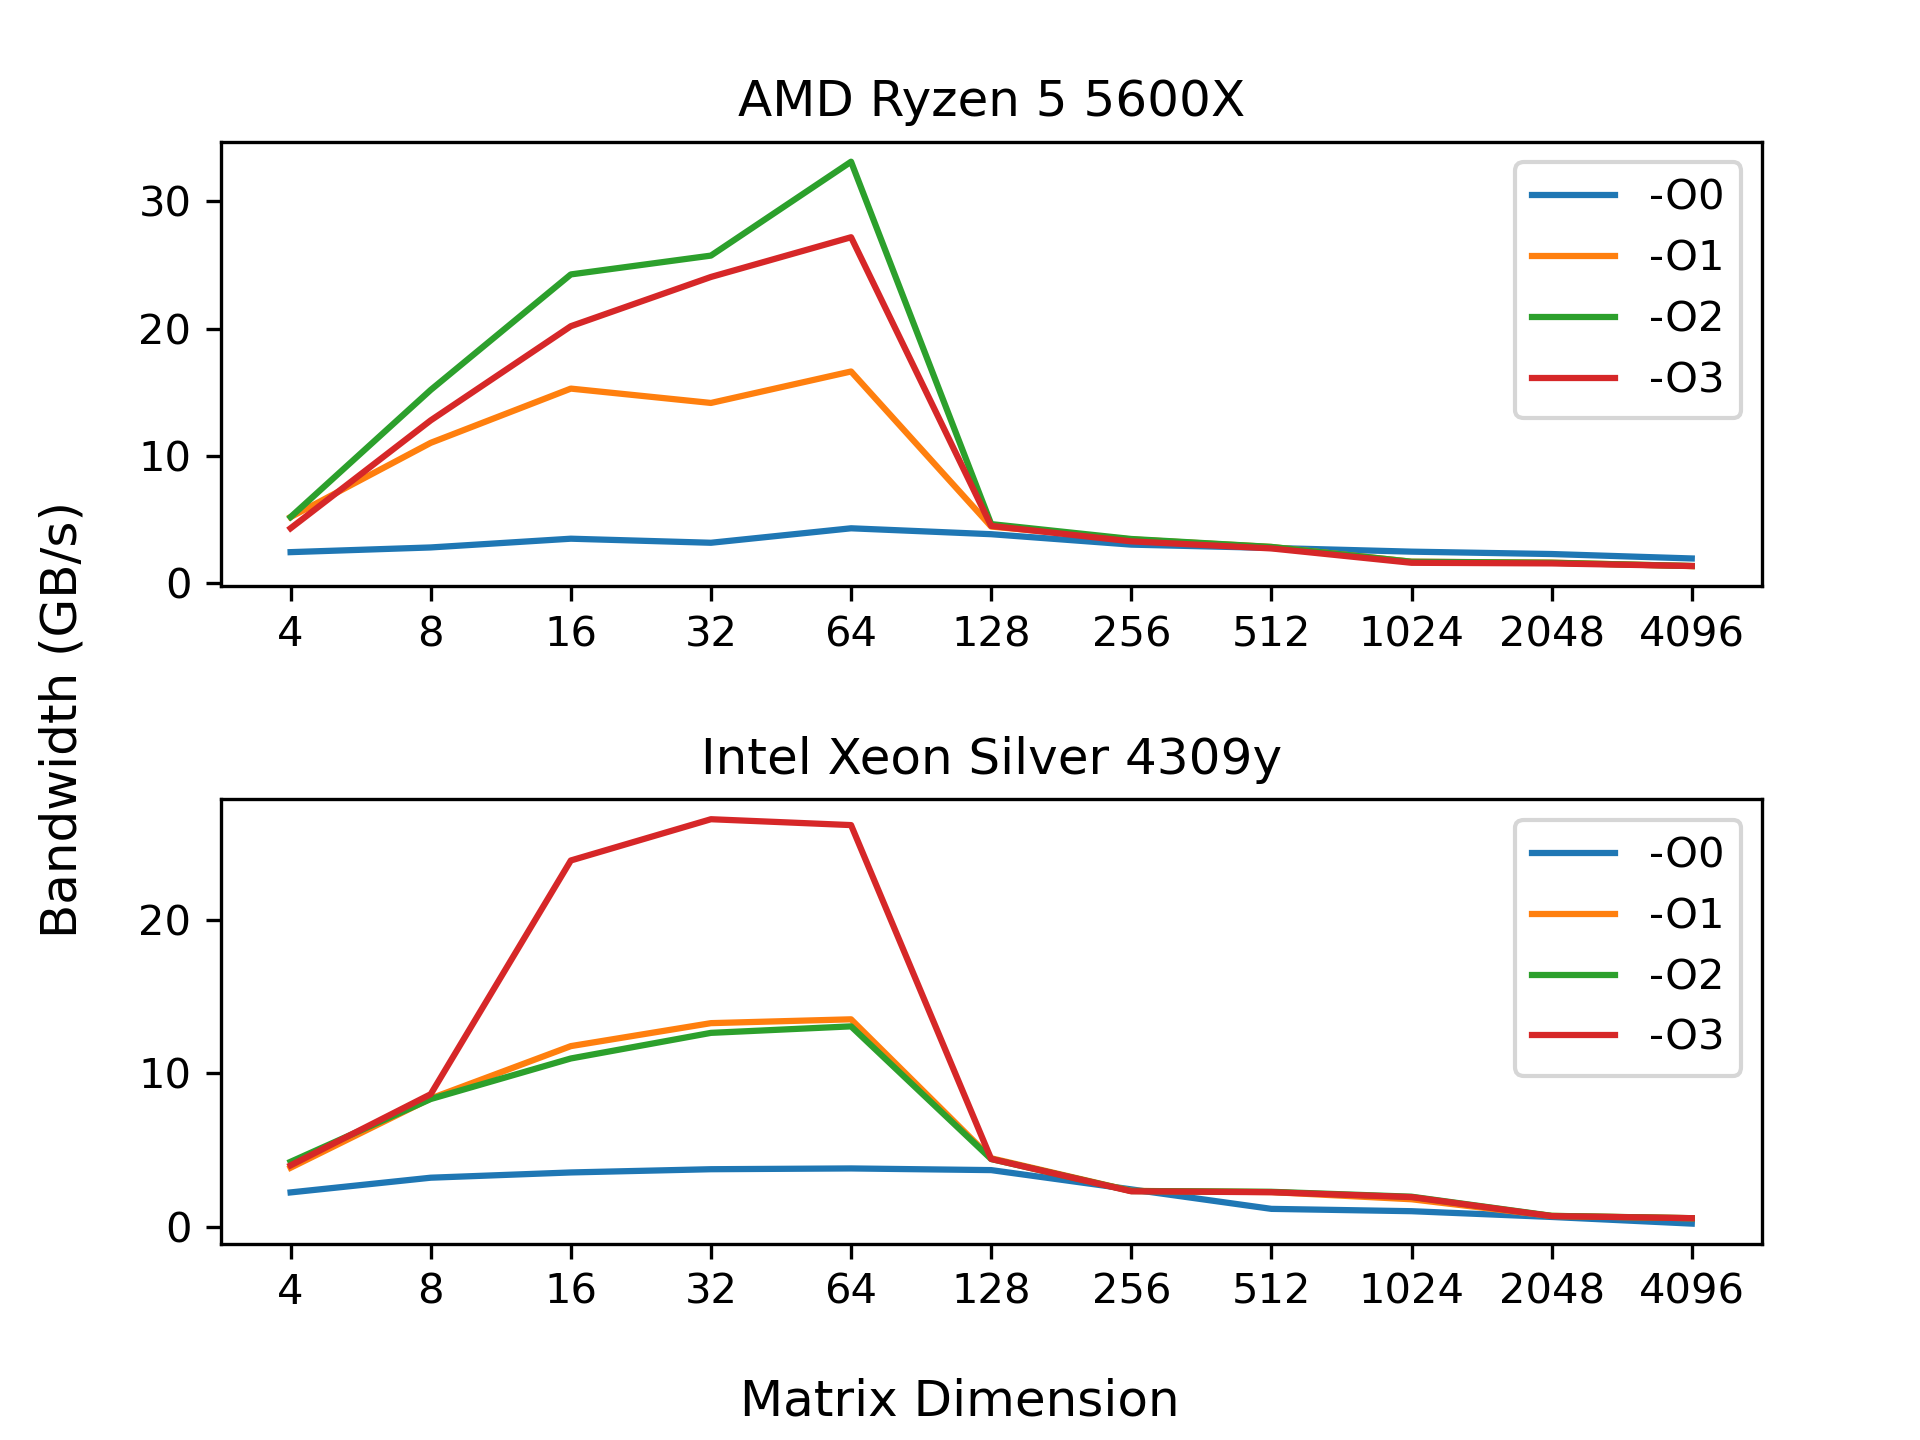
\includegraphics[scale=0.8]{report/img/naive_comparison.png}
    \caption{Comparison of the na\"{i}ve matrix transposition algorithm}
    \label{fig:naive_comparison}
\end{figure}
\subsubsection{Blocked Algorithm}
The idea behind the blocked algorithm is to reduce the number of cache misses by exploiting the locality of the data. But in order to benefit from this the block
size must be chosen with care, since it also depends on the size of the cache line. Different dimensions have been used to test the algorithm and find the best one.
In this step, we used a matrix of $1024 \times 1024$ and set the optimization flag to \texttt{-O3}.
The results for the used platforms are shown in table \ref{tab:blocked_results}, where the highlighted rows indicate the most appropriate 
block size for the given processor. \\
Subsequently, as shown in figure \ref{fig:blocked_comparison}, the results are pretty evident. Indeed, the blocked algorithm outperforms the na\"{i}ve one on both platforms. \\
The cache miss rate analysis highlights how the blocked algorithm is able to exploit the temporal locality of the data.
The results of the analysis are shown in table \ref{tab:blocked_cache_miss}. \\

\begin{table}[h]
    \centering
    \begin{tabular}{|c|c|}
        \hline
        \multicolumn{2}{|c|}{\textbf{Ryzen 5 5600X}} \\
        \hline
        \textbf{Blocksize } & \textbf{Bandwidth (GB/s)} \\ \hline
        2         & 4.85 \\ \hline
        \rowcolor{LightYellow}
        4         & 7.49 \\ \hline
        8         & 3.47 \\ \hline
        16        & 3.62 \\ \hline
        32        & 3.33 \\ \hline
        64        & 2.75 \\ \hline
    \end{tabular}
    \hspace{2em}
    \begin{tabular}{|c|c|}
        \hline
        \multicolumn{2}{|c|}{\textbf{Xeon 4309y}} \\
        \hline
        \textbf{Blocksize } & \textbf{Bandwidth (GB/s)} \\ \hline
        2         & 2.04 \\ \hline
        4         & 3.83 \\ \hline
        \rowcolor{LightYellow}
        8         & 4.80 \\ \hline
        16        & 2.45 \\ \hline
        32        & 2.59 \\ \hline
        64        & 2.72 \\ \hline
    \end{tabular}
    \caption{Results of the blocked algorithm with different block sizes ($1024 \times 1024$, \texttt{-O3})}
    \label{tab:blocked_results}
\end{table}
\begin{figure}[H]
    \centering
    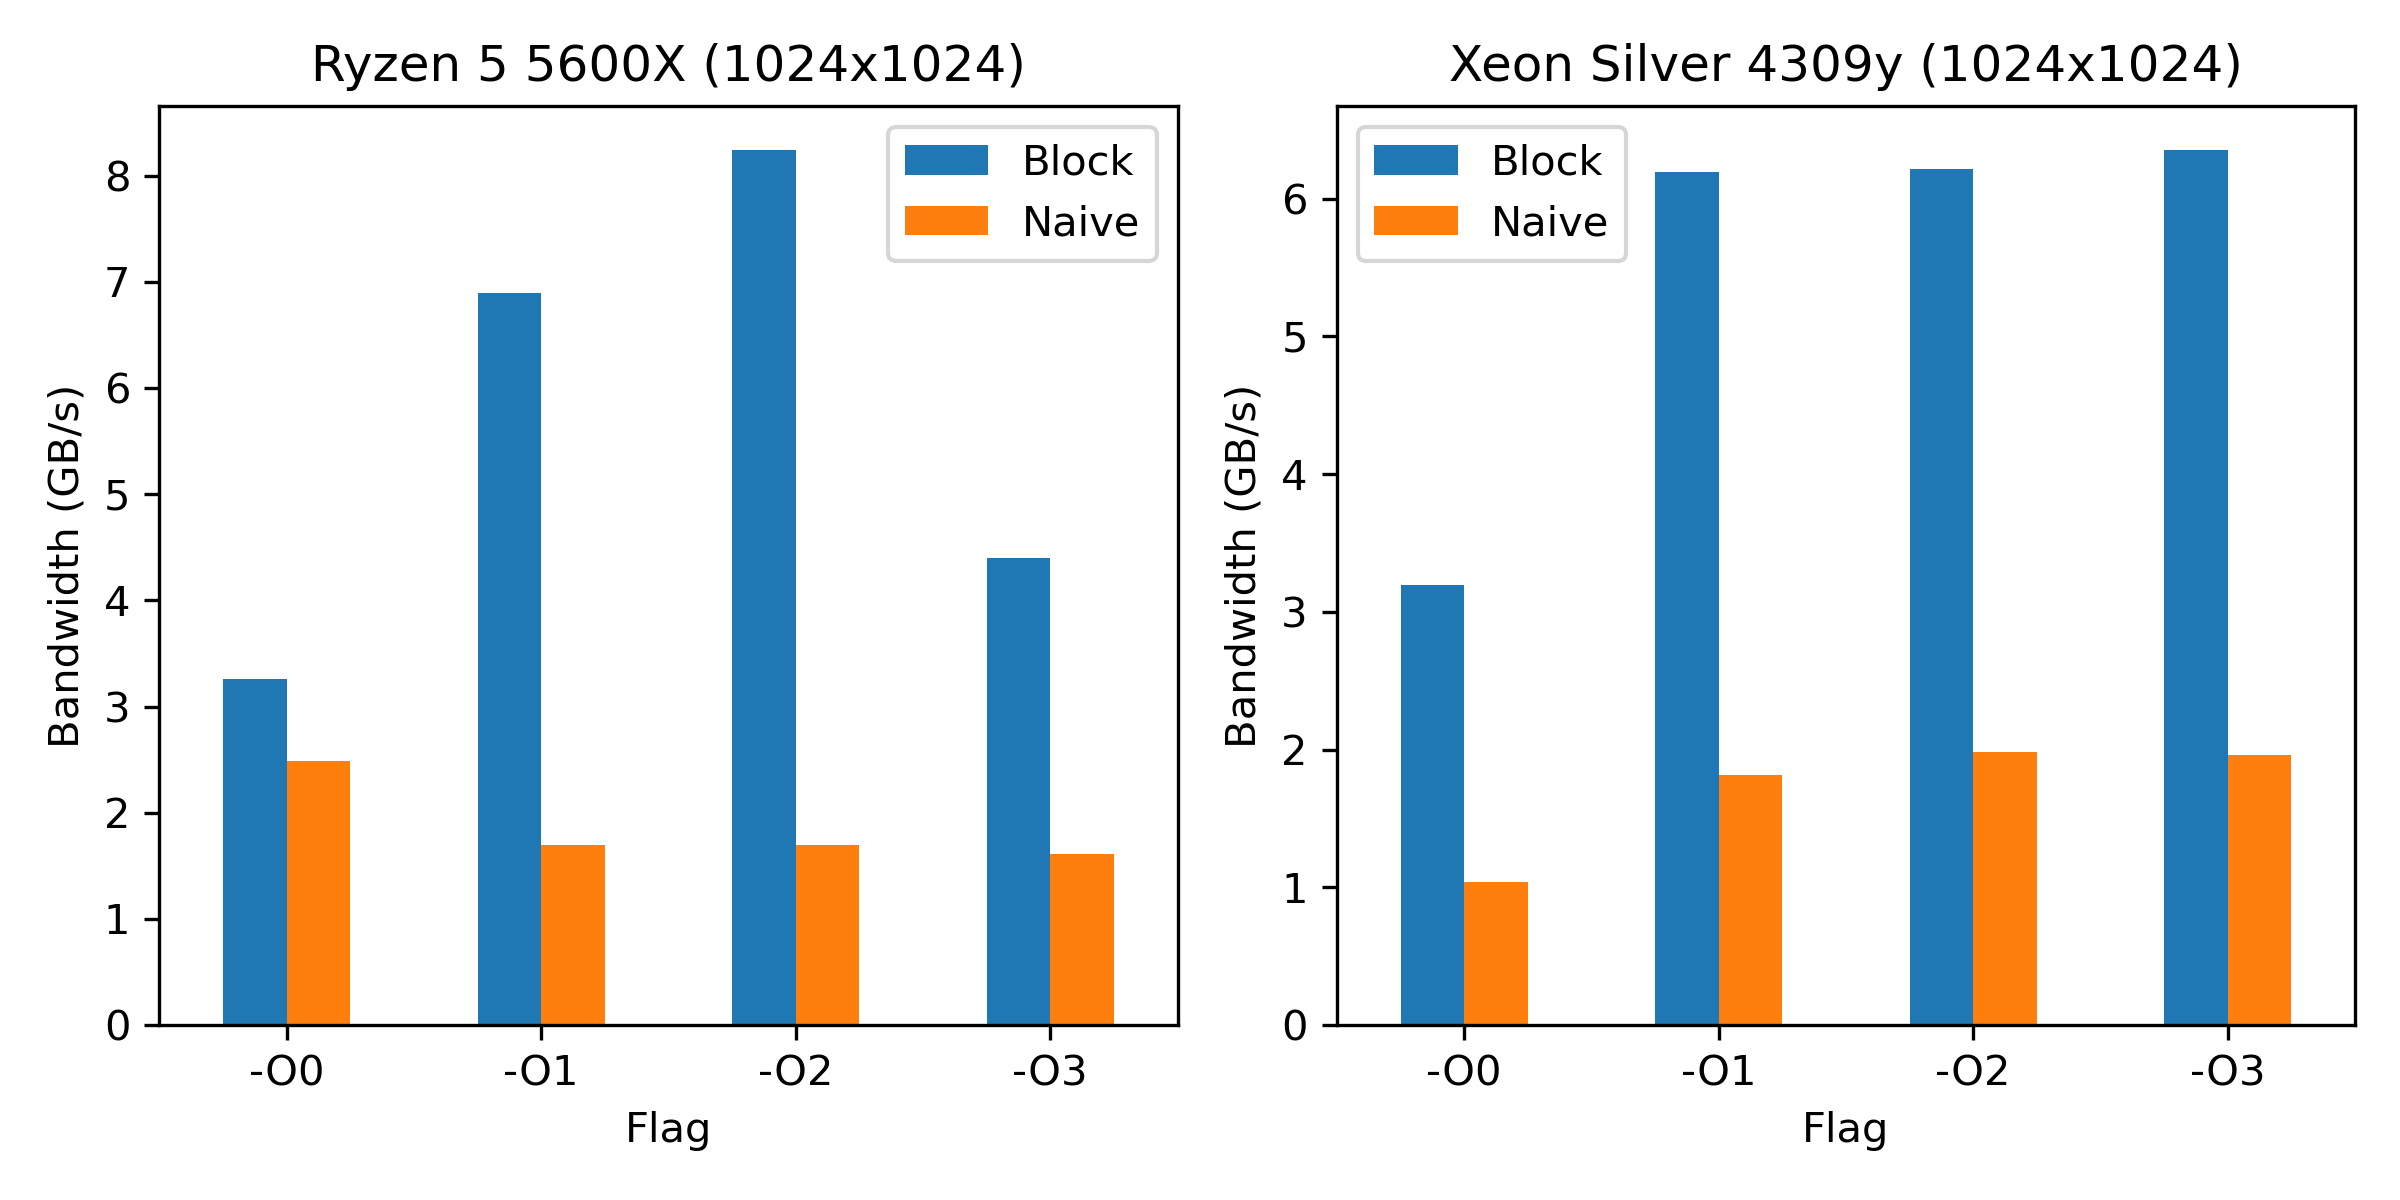
\includegraphics[width=0.85\textwidth]{report/img/block_vs_naive.png}
    \caption{Comparison of the blocked algorithm against the na\"{i}ve algorithm}
    \label{fig:blocked_comparison}
\end{figure}
\begin{table}[h]
    \centering
    \begin{tabular}{|c|c|c|c|}
        \hline
        \multicolumn{4}{|c|}{\textbf{Ryzen 5 5600X}} \\ 
        \hline
        \textbf{Algorithm} & \textbf{Dimension} & \textbf{I1 m.r.} & \textbf{D1 m.r}. \\ \hline
        Na\"{i}ve & 1024        & 0.00\%       & 4.0\%        \\ \hline
        Blocked  & 1024        & 0.00\%       & 1.4\%        \\ \hline
    \end{tabular}
    \hspace{2em}
    \begin{tabular}{|c|c|c|c|}
        \hline
        \multicolumn{4}{|c|}{\textbf{Xeon 4309y}} \\ 
        \hline
        \textbf{Algorithm} & \textbf{Dimension} & \textbf{I1 m.r.} & \textbf{D1 m.r}. \\ \hline
        Na\"{i}ve & 1024        & 0.01\%       & 3.7\%        \\ \hline
        Blocked  & 1024        & 0.00\%       & 1.0\%        \\ \hline
    \end{tabular}
    \caption{Comparison of the cache miss rate between the na\"{i}ve and the blocked algorithm, \texttt{-O3}}
    \label{tab:blocked_cache_miss}
\end{table}
\section{Conclusion}
To conclude, if provided with an adequate block size, the blocked algorithm is able to achieve an higher effective bandwidth than the na\"{i}ve one.
These results are concordant with the outcomes of the cache analysis. \\
A future direction to further improve the performance could be to parallelize the algorithms. A possible solution could ideally employ the usage of one thread 
for each cell of the matrix. Of course, this approach would require a high number of threads, therefore being impractical for large matrices. Instead, a better solution 
could be to divide the matrix into blocks and assign a thread to each of them.
\end{document}

